\documentclass[pdftex]{article}
\usepackage[T1]{fontenc}
\usepackage[utf8]{inputenc}
\usepackage{graphicx}
\usepackage[font=scriptsize,labelfont=bf]{caption}
\usepackage{titling}

\setlength{\droptitle}{-15em}
\title{PHYS 723 Homework 8}
\author{Nick Tyler}
\date{}


\begin{document}
\captionsetup[figure]{aboveskip=-15pt}
\captionsetup[figure]{belowskip=15pt}
\maketitle
\begin{enumerate}
	\item  The CKM matrix triangle representation with axes of $\bar{\eta}$ and $\bar{\rho}$.  
	The values for $\bar{\eta}$ and $\bar{\rho}$, as well as their errors were found on the CKM fitter website. 
	[http://ckmfitter.in2p3.fr] \\
	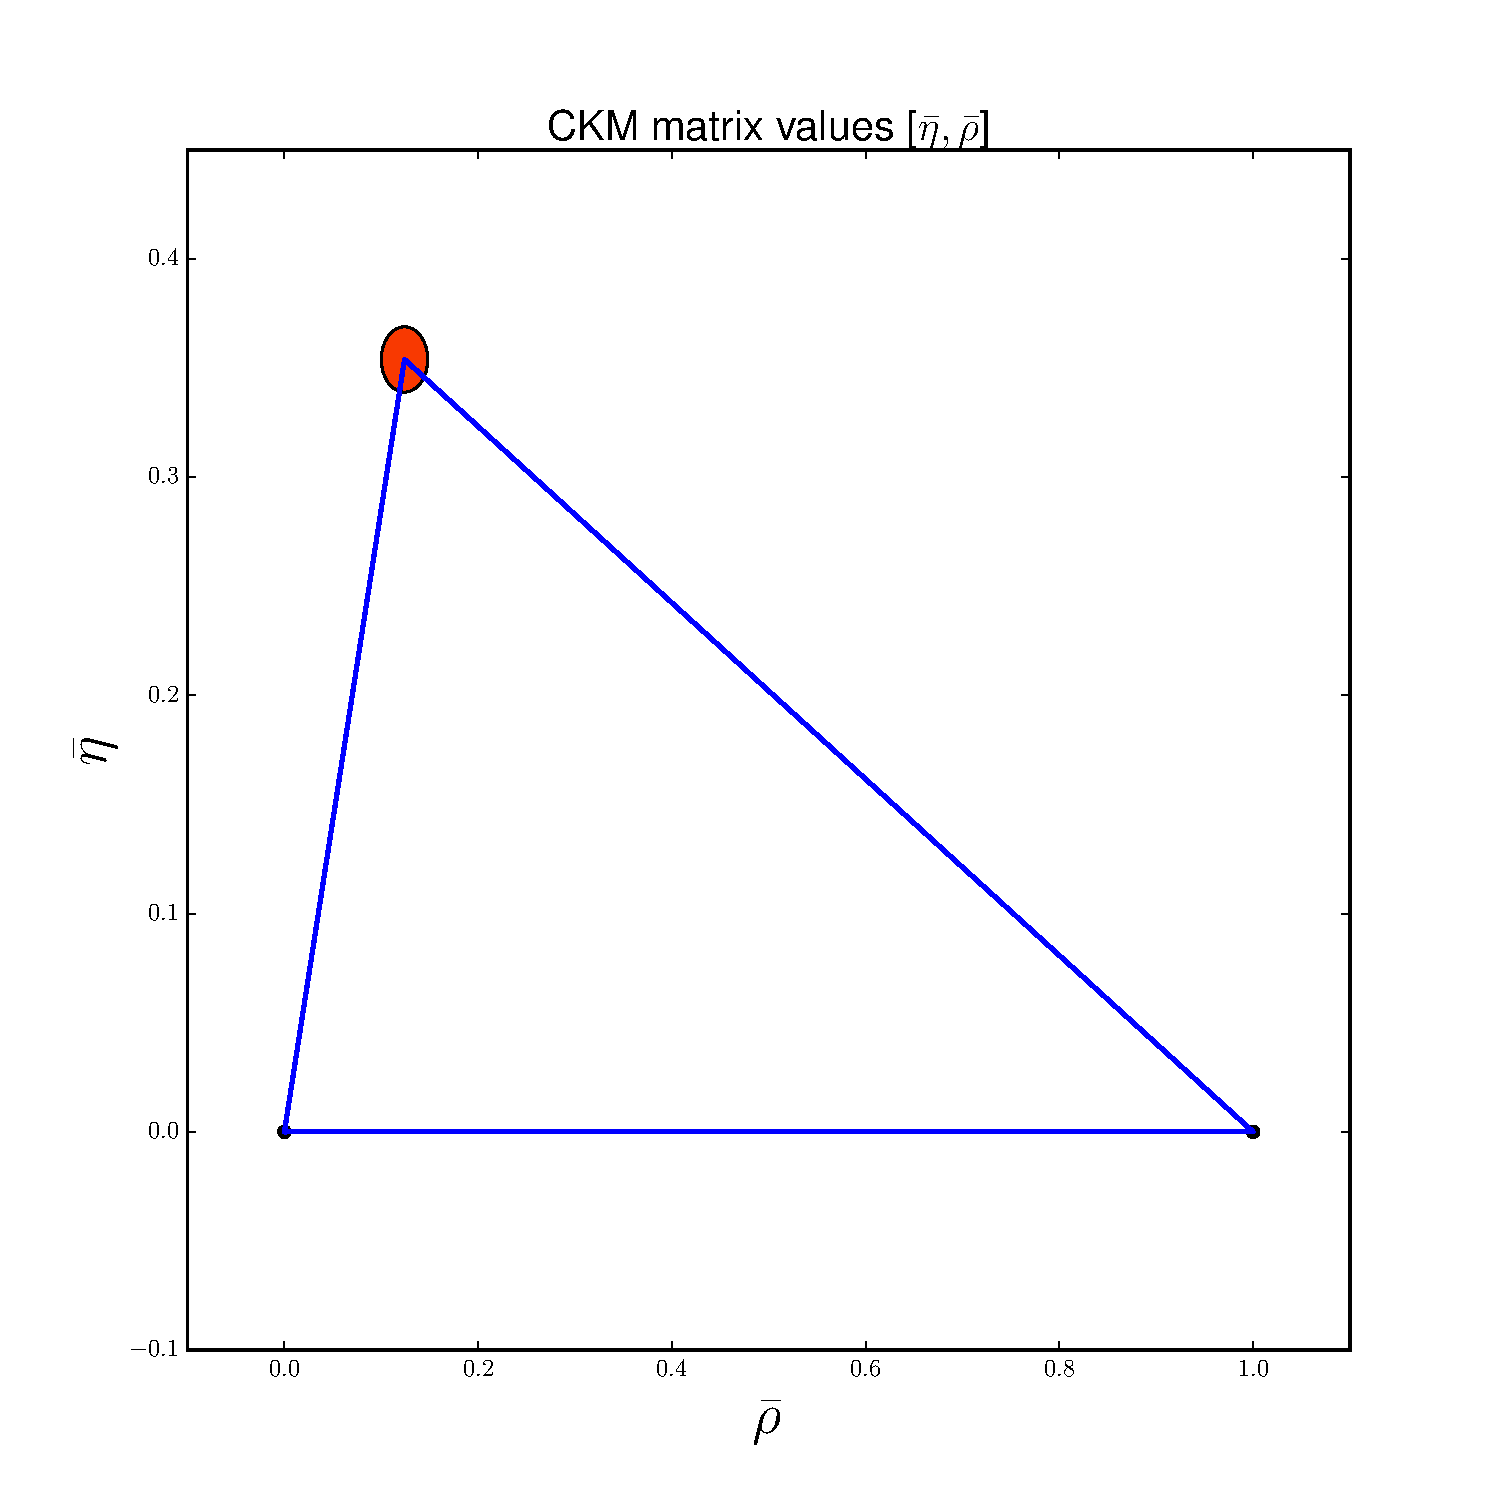
\includegraphics[scale=0.4]{CKMTri.pdf}\\
	\captionof{figure}{Values for $\bar{\eta}$ and $\bar{\rho}$ plotted with error ellipse.}



\end{enumerate}

\end{document}
